\chapter{Graph Matching}
\label{chap: graphmatching}

\section{Introduction}

In order to extract the common pattern from graphs, we need to first compare two graphs and match\footnotemark the relevant part together to better summarize them. However, since the largest common subgraph problem is NP-complete, the graph matching problem we are dealing with is also NP-complete (even though you can argue it's NP-hard in some other definition). Therefore, we must look for good suboptimal solutions via approximation.
\footnotetext{The graph matching here is different than the "matching" problem in graph theory where the \emph{matching} is a set of pairwise non-adjacent edge.}\\

There are two main approaches for graph matching. One approach involves the construction of a state-space that can be searched via some brach and bound methods. While some heuristic rule can help us reduce the complexity from exponential to polynomial, the polynomial complexity would still have a high complexity. The second approach employs nonlinear optimization methods like relaxation labeling, which do not search based on the state-space and generally have a much lower computational complexity.\\

In the realm of nonlinear optimization methods and similar to relaxation labeling, here we described a graduated assigned approach developed by Gold and Rangarajan in 1996 and the improvement we made on the algorithm in order deal with larger graphs we encounter today 20 years later.

\section{Syntax and Definition}

Here we use a attributed relational graph (ARG) to represent our spatial pattern. An ARG, $G$, is a \emph{directional} graph with labels on its nodes ($\overrightarrow{N_{a}}$ is the label for the $a$th node in the graph) and edges ($\overrightarrow{E_{ab}}$ is the label for the edge from the $a$th node to the $b$th node). \\

Since two graphs might only match partially by their subgraph or might not have match at all, Gold and Rangarajan add a null node, $\phi$, in each ARG.\\

We then can define the node compatibility function($c_N$) and the edge compatibility function($c_E$) to calculate the compatibility, $C$, between the nodes and edges between two ARGs, $G$ and $G'$. Here, $C_{ai}$ is the compatibility between node $\overrightarrow{N_{a}}$ in $G$ and node $\overrightarrow{N_{i}}$ in $G'$, while $C_{abij}$ is the compatibility between edge $\overrightarrow{E_{ab}}$ in $G$ and $\overrightarrow{E_{ij}}$ in $G'$.\\

The match result is defined as a matrix $M$ where $M_{ai}$ is the probability matching the $a$th node in $G$ to the $i$th node in $G'$.

\section{Problem Definition}

We defined the problem of ARG matching in the following manner. Given two ARG, $G$ and $G'$, we want to find the match matrix $M$ such that the following objective function is minimized:

\begin{equation}\label{eq:energy}
E(M)=-\frac{1}{2}\sum_{a=1}^{G}\sum_{i=1}^{G'}\sum_{b=1}^{G}\sum_{j=1}^{G'}M_{ai}M_{bj}C_{abij}-\alpha\sum_{a=1}^{G}\sum_{i=1}^{G'}M_{ai}C_{ai}
\end{equation}
subject to a two way constraints: $\forall a\ne\phi$, $\sum_{i=1}^{G'}M_{ai}=1$ and $\forall i\ne\phi$, $\sum_{i=1}^GM_{ai}=1$:

\begin{figure}[h]
	\centering
	\captionsetup{justification=centering}
	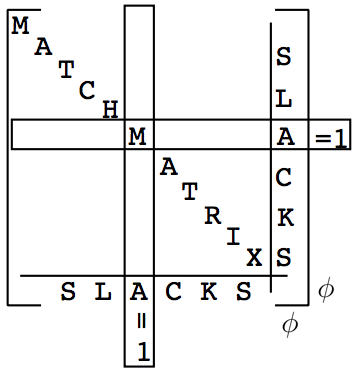
\includegraphics[width=0.25\textwidth]{figs/two_way_constraints.png}
	\caption[Caption for LOF]{\emph{Both rows and columns should sum up to 1 except the row and column involving $\phi$ nodes, which are considered the slack row and slack column.}}
	\label{fig:two_way_constraints}
\end{figure}

\section{Graph Matching by Gold and Rangarajan}

In Gold and Rangarajan's original algorithm, they solve the problem using a graduated assignment method where the two-way constraints are satisfied by normalizing rows and columns iteratively for many rounds (Sinkhorn 1963) and their compatibilities are defined as:
\begin{align} 
& C_{ai}  = \begin{cases}0 & a=\phi \bigcup i=\phi \\c_N(\overrightarrow{N_{a}},\overrightarrow{N_{i}}) & otherwise\end{cases}\\
& C_{abij} = \begin{cases}0 & a=\phi \bigcup b=\phi \bigcup i=\phi \bigcup j=\phi \\c_E(\overrightarrow{E_{ab}},\overrightarrow{E_{ij}}) & otherwise\end{cases} 
\end{align}\\

To expand on their graduated assignment method, we will first need to convert our objective function to an assignment problem. They way we do it is through Taylor series approximation, where given an initial $M^0$, we would have:
\begin{align}
E(M) = & -\frac{1}{2}\sum_{a=1}^{G}\sum_{i=1}^{G'}\sum_{b=1}^{G}\sum_{j=1}^{G'}M_{ai}M_{bj}C_{abij}-\alpha\sum_{a=1}^{G}\sum_{i=1}^{G'}M_{ai}C_{ai}\nonumber\\
= & -\frac{1}{2}\sum_{a=1}^{G}\sum_{i=1}^{G'}\sum_{b=1}^{G}\sum_{j=1}^{G'}M_{ai}^{0}M_{bj}^{0}C_{abij}-\alpha\sum_{a=1}^{G}\sum_{i=1}^{G'}M_{ai}^{0}C_{ai} - Q_{ai}(M_{ai}-M_{ai}^{0})
\end{align}
where
\begin{equation} 
Q_{ai}=-\frac{\partial E}{\partial M_{ai}}\bigg\rvert_{M=M_0}=+\sum_{b=1}^{G}\sum_{j=1}^{G'}M_{bj}^{0}C_{abij}+\alpha C_{ai}
\end{equation}\\

Therefore, minimizing our objective function $E$ based on our Taylor series expansion is equivalent to maximizing 
\begin{equation}
+\sum_{a=1}^{G}\sum_{i=1}^{G'}Q_{ai}M_{ai}
\end{equation}
which is an assignment problem!\\

Therefore, we can run the following algorithm for the graduated assignment:\\
\\
\textbf{Initialize} $\beta$ to $\beta_{0}$, $M_{ai}$ to a random sample from $U(0,1)$\\
\textbf{Begin $A$:} (Do $A$ until $\beta \geq \beta_{f}$)\\
\indent \textbf{Begin $B$:} (Do $B$ until $M$ converges or \# of iterations $>I_0$)\\
\indent $Q_{ai} \leftarrow \sum_{b=1}^{G}\sum_{j=1}^{G'}M_{bj}^{0}C_{abij}+\alpha C_{ai}$\\
\indent $M_{ai}^{0} \leftarrow exp(\beta Q_{qi})$\\
\indent \indent \textbf{Begin $C$:} (Do $C$ until $M$ converges or \# of iterations $>I_1$)\\
\indent \indent  Update $M$ by normalizing across all rows:\\
\indent \indent  $M_{ai}^{1}=\frac{M_{ai}^{0}}{\sum_{i=1}^{G'}M_{ai}^{0}}$ for all $a\neq\phi$\\
\indent \indent  Update $M$ by normalizing across all columns:\\
\indent \indent  $M_{ai}^{0}=\frac{M_{ai}^{1}}{\sum_{a=1}^{G}M_{ai}^{1}}$ for all $i\neq\phi$\\
\indent \indent \textbf{End $C$}\\
\indent \textbf{End $B$}\\
$\beta\leftarrow\beta_{r}\beta$\\
\textbf{End $A$}\\
\textbf{Perform Clean-up Heuristic}\\

Variable and constant definitions can be found as:
\begin{figure}[h]
	\centering
	\captionsetup{justification=centering}
	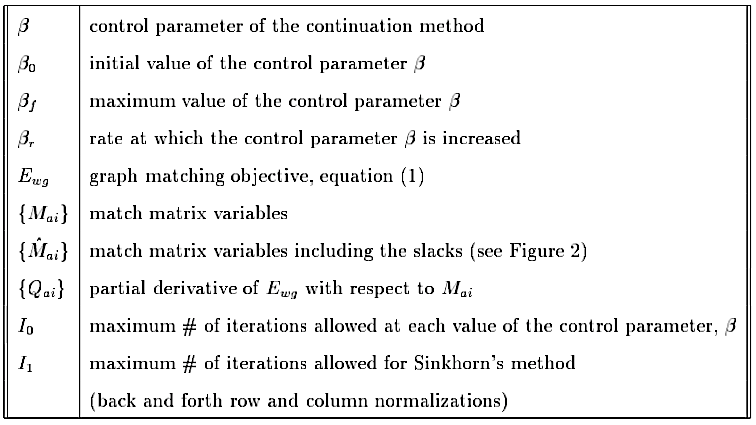
\includegraphics[width=0.95\textwidth]{figs/algorithm_variable.png}
\end{figure}

\section{Implementation Detail}

\subsection{Compatibility}
\label{ssec:compatibility}

To calculate the compatibility, we assume the label/feature follows a Gaussian probability distribution function so that the compatibility function $c_N$ and $c_G$ is defined as:
\begin{equation} 
c_N( \overrightarrow{a}, \overrightarrow{b} )=c_E( \overrightarrow{a}, \overrightarrow{b})=\frac{exp(-\frac{1}{2}(\overrightarrow{a}-\overrightarrow{b})^{T}\Sigma^{-1}(\overrightarrow{a}-\overrightarrow{b})}{(2\pi)^{\zeta/2}|\Sigma|^{1/2}}
\end{equation}
where $\delta$ is the covariance matrix and $\zeta$ is the dimension of $\overrightarrow{a}$ and $\overrightarrow{b}$. Since we assume feature independence, the covariance matrix $\delta$ is the identity matrix, which essentially will give us:
\begin{equation} 
c_N( \overrightarrow{a}, \overrightarrow{b} )=c_E( \overrightarrow{a}, \overrightarrow{b})=\frac{exp(-\frac{1}{2}(\overrightarrow{a}-\overrightarrow{b})^{T}(\overrightarrow{a}-\overrightarrow{b})}{(2\pi)^{\zeta/2}}
\end{equation}

\subsection{Parallel Computing and Caching}

The majority of the computation complexity in the algorithm is in computing the compatibility, especially the edge compatibility.\\

Since the compatibility function defined can be computer independently, one way we could speed up the algorithm is calculating the compatibility in parallel fashion.\\

Another way we could improve the computation time would be through caching, where we can pre compute a node and edge compatibility matrix, as the label is never updated. However, the edge compatibility matrix can be very large and takes a lot of memory to cache, so you might also want to use data structure like \emph{sparse matrix} since the connection matrix (representing edge) is likely to be sparse as well.

\subsection{Heuristic}

In our implementation, we use a very simple heuristic to clean up the match matrix $M$ from a \emph{softassign} matrix to a matrix only with $0$ and $1$. We simply set the largest value (at index $j$) for each row $i$ to 1 and other value to 0. After setting $M_{ij}$ to 1, we also set the entire $j$ column to 0 in order to satisfy the two-way constraints.\\

If you want to be more fancy about this, you can also convert this heuristic problem to a maximum spanning tree problem to make sure all the $M_{ij}$ that you set to 1 have the largest sum.

\subsection{Converge Condition}

In our implementation, we compare the previous match matrix $M^{(0)}$ and the current match matrix $M^{(1)}$, and conclude the matrix converge if the difference is less than some threshold $\iota$:

\begin{equation} 
\sum_{a=1}^{G}\sum_{i=1}^{G'}|M_{ai}^{(0)}-M_{ai}^{(1)}|<\iota
\end{equation}

\subsection{Run Time}
\label{ssec:graphmatchingruntime}

The algorithm takes $\sim15s$ to complete when matching two graphs with $\sim30$ nodes. However, you can certainly adjust the parameter like $I$ and $\beta$ to achieve faster run time.

\section{Testing the Algorithm}
\label{sec:graphmatchingtest}

To test the algorithm, we first set a noise level $\epsilon \in [0,1]$. Then we generate a pattern with $n$ nodes and embed this pattern to $2$ randomly generated graphs, $G$ and $G'$, with $n$ to $n*(1+\epsilon)$ nodes. Once we embed the pattern in these two random graphs, we shuffle the index for each node and add some noise to the node and edge labels:

\begin{equation} 
\overrightarrow{N_{a}} \leftarrow \overrightarrow{N_{a}}  + \chi*\overline{N} \text{ where } \chi \in [0,\epsilon]
\end{equation}
\begin{equation} 
\overrightarrow{E_{ab}} \leftarrow \overrightarrow{E_{ab}}  + \chi*\overline{E} \text{ where } \chi \in [0,\epsilon]
\end{equation}\\

We then run the matching algorithm $match(G,G')$ and get a match matrix $M$. We ignore the match with the null node $\phi$, and calculate the total number of correct match $m$, and the total number of match observed $l$ from the match matrix $M$. Then we can evaluate the performance by $precision$, $recall$ and $F_1 score$:
\begin{align} 
& precision = \frac{m}{l}\\
& recall = \frac{m}{n}\\
& F_1 =2*\frac{precision*recall}{precision+recall}
\end{align}

\section{Improvement and Modification}

While the original algorithm works well with small graphs with 20 to 30 nodes, we run into some problems while matching larger graphs with 50 to 100 nodes and therefore make some improvement to Gold and Rangarajan's original algorithm.

\subsection{Local Minima}

The first problem we encounter is local minima. In this case, the algorithm will generate correct and even perfect match for majority of the test cases. However, for some of the test case, the match result is entirely wrong, which indicates that the graduated assignment process stuck in some local minima.\\

In the original algorithm, if we initialized $M_0$ in the wrong places, the assignment process can easily get stuck in sub-optimal match (local minima). While adjusting $\beta$ and $\beta_r$ can mediate the problem, it does not work well in larger graphs since there are more sub-optimal match. Therefore, we introduce a stochastic process in the algorithm:

\begin{figure}[h]
	\centering
	\captionsetup{justification=centering}
	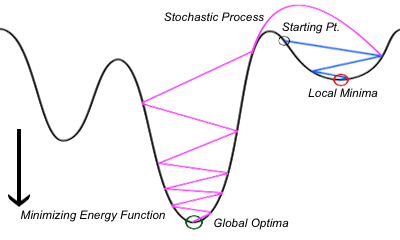
\includegraphics[width=0.46\textwidth]{figs/stochastic.png}
	\caption[Caption for LOF]{\emph{The intuition behind introducing the stochastic process.}}
	\label{fig:stochastic}
\end{figure}

In the stochastic process, we essentially add some small noise to the match matrix at the beginning of step \textbf{$B$}:
\begin{equation} 
M_{ai}^{0} \leftarrow M_{ai}^{0} + \frac{\tau * U(-1,1)}{|G|}
\end{equation}
where $\tau$ is the stochastic/noise level, $|G|$ is the number of node in $G$, and $U(-1,1)$ is a random sample from a uniform distribution between $-1$ and $+1$.\\

Therefore, the updated algorithm becomes:\\
\\
\textbf{Initialize} $\beta$ to $\beta_{0}$, $M_{ai}$ to a random sample from $U(0,1)$\\
\textbf{Begin $A$:} (Do $A$ until $\beta \geq \beta_{f}$)\\
\indent \textbf{Begin $B$:} (Do $B$ until $M$ converges or \# of iterations $>I_0$)\\
\indent \textcolor{red}{$M_{ai}^{0} \leftarrow M_{ai}^{0} + \frac{\tau * U(-1,1)}{|G|}$}\\
\indent $Q_{ai} \leftarrow \sum_{b=1}^{G}\sum_{j=1}^{G'}M_{bj}^{0}C_{abij}+\alpha C_{ai}$\\
\indent $M_{ai}^{0} \leftarrow exp(\beta Q_{qi})$\\
\indent \indent \textbf{Begin $C$:} (Do $C$ until $M$ converges or \# of iterations $>I_1$)\\
\indent \indent  Update $M$ by normalizing across all rows:\\
\indent \indent  $M_{ai}^{1}=\frac{M_{ai}^{0}}{\sum_{i=1}^{G'}M_{ai}^{0}}$ for all $a\neq\phi$\\
\indent \indent  Update $M$ by normalizing across all columns:\\
\indent \indent  $M_{ai}^{0}=\frac{M_{ai}^{1}}{\sum_{a=1}^{G}M_{ai}^{1}}$ for all $i\neq\phi$\\
\indent \indent \textbf{End $C$}\\
\indent \textbf{End $B$}\\
$\beta\leftarrow\beta_{r}\beta$\\
\textbf{End $A$}\\
\textbf{Perform Clean-up Heuristic}\\

Once we incorporate the stochastic process to the algorithm, we gain a significant improvement in $F_1$ score and there is very little chance the match result is entirely wrong:

\begin{figure}[h]
	\centering
	\captionsetup{justification=centering}
	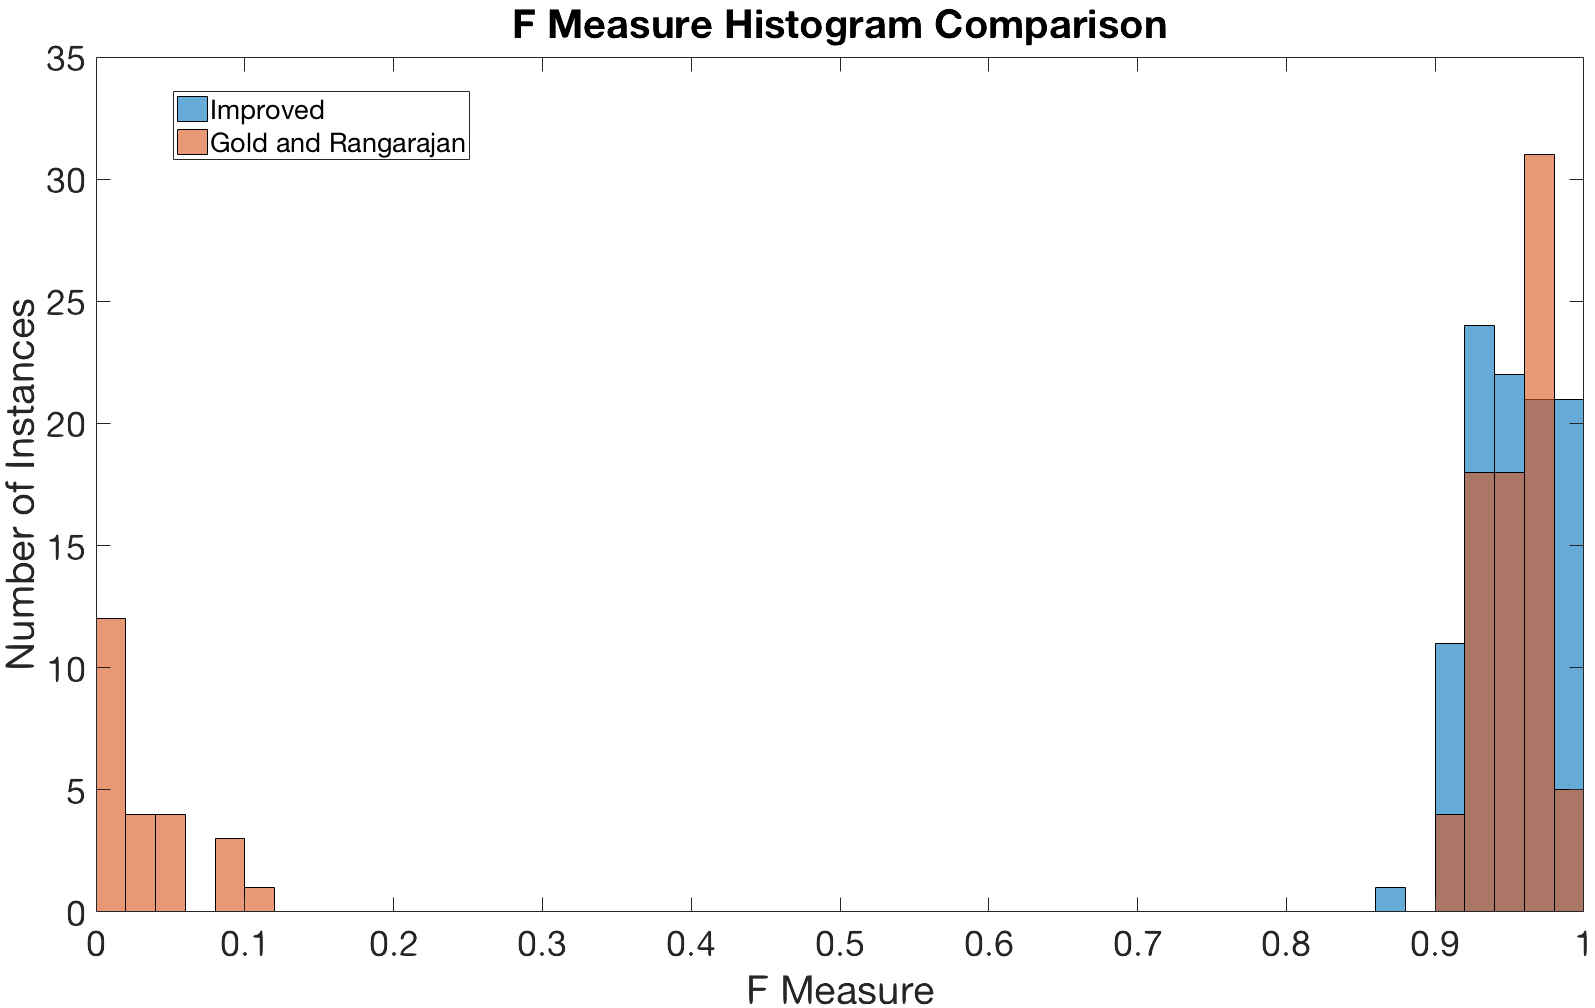
\includegraphics[width=0.85\textwidth]{figs/s_improved.png}
	\caption[Caption for LOF]{\emph{$F_1$ score distribution histogram for the original algorithm (orange) and the improved algorithm with stochastic process (blue).}}
	\label{fig:s_improved}
\end{figure}

\subsection{High Recall + Low Precision}
\label{ssec:nullnode}

The other challenge we encounter is that even though we get high recall rate in a test, we also get low precision rate, which means the algorithm can generate correct match but also force many of the background nodes (i.e. nodes outside of the pattern) matching  to each other.\\

The first explanation came across our mind would be the two test graphs we generated can share pattern outside the embedded one. However, after careful examination, this is proven not the case.\\

Therefore, we examed how Gold and Rangarajan's original algorithm matches background nodes in $G$ to the null node $\phi$ in $G'$. We realized that since the original algorithm define the compatibility function so that any compatibility related to the $\phi$ node will be set to 0. Therefore, the algorithm does not \emph{actively} match background nodes to  $\phi$ node, but \emph{hope} that the background noise does not attract to one specific node, and end up matching with the $\phi$ node.\\

To handle this problem gracefully, we essentially want to create a fully connected null node network that can match to any of the background pattern. Therefore, we rewrite the compatibility function as:

\begin{align} 
& C_{ai}  = \begin{cases}
0 & a,i=\phi \\
c_N(\overrightarrow{N_{a}},\overrightarrow{N_{i}}) & a, i\neq\phi \\
p \text{ percentile of }[C_{1i}, C_{2i},...C_{|G|-1i}] & a=\phi\\
p \text{ percentile of }[C_{a1}, C_{a2},...C_{a|G'|-1}] & i=\phi
\end{cases}\\
& C_{abij} = \begin{cases}
c_E(\overrightarrow{E_{ab}},\overrightarrow{E_{ij}})  & a,b,i,j\neq\phi \\
p \text{ percentile of }\{C_{abij}|a,b,i,j\neq\phi\} & a,b\neq\phi \bigcap i,j=\phi\\
p \text{ percentile of }\{C_{abij}|a,b,i,j\neq\phi\} & a,b=\phi \bigcap i,j\neq\phi\\
0 & otherwise\\
\end{cases}
\end{align}
where $p$ is a percentile we can adjust so that set to 100 to give null node/edge the maximum compatibility every seen while set to 0 to give the minimum compatibility. You can adjust the $p$ to balance the recall and precision rate since higher percentile will encourage nodes match to null node result in low recall but high precision while lower percentile will allow background nodes match together result in high recall but low precision.\\

While this is a lot to unpack, the updated compatibility function essentially create a self-linked edge for null node $\overrightarrow{E_{\phi\phi}}$ and give definition for the compatibility of null node to other real node and self-linked null edge to other edge linking two real nodes. Since we don't normalized the slack row and column (match result for null node), this is equivalent to create a fully connected null node network:

\begin{figure}[h]
	\centering
	\captionsetup{justification=centering}
	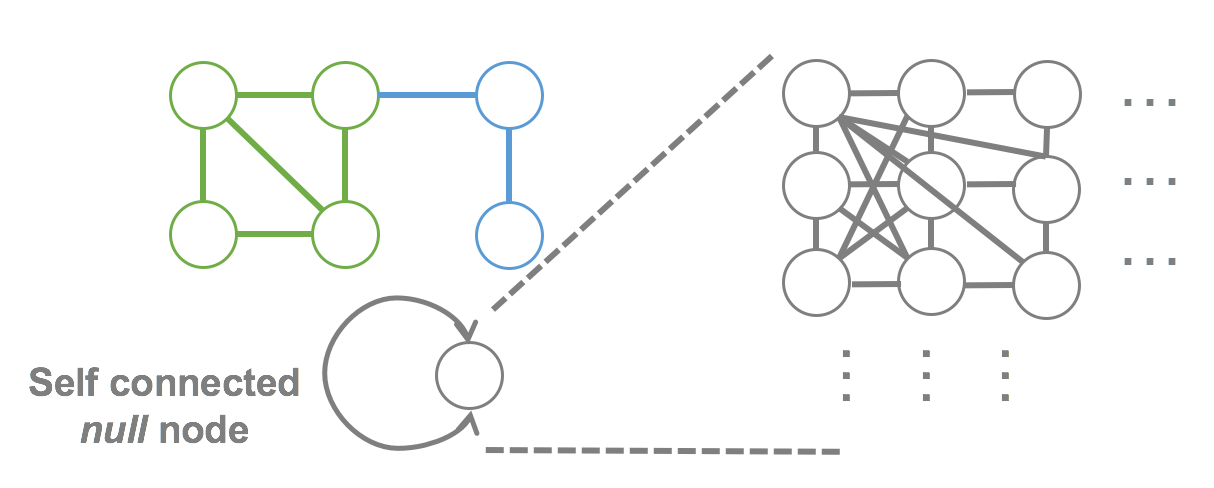
\includegraphics[width=0.46\textwidth]{figs/null_node_network.png}
	\caption[Caption for LOF]{\emph{The self linked/connected null node $\phi$ (grey) can be treated as a fully connected null node that can be matched to any pattern including background nodes. }}
	\label{fig:null_node_network}
\end{figure}

After modified the compatibility function in the original algorithm, we are able to generate match result with both high recall and high precision. For instance, two graph with backgrounds nodes at the beginning and the end (in terms of their index) are not forced to match to each other (left) and end up match to the null node/the slack column/row in the end (right):
\begin{figure}[h]
	\centering
	\captionsetup{justification=centering}
	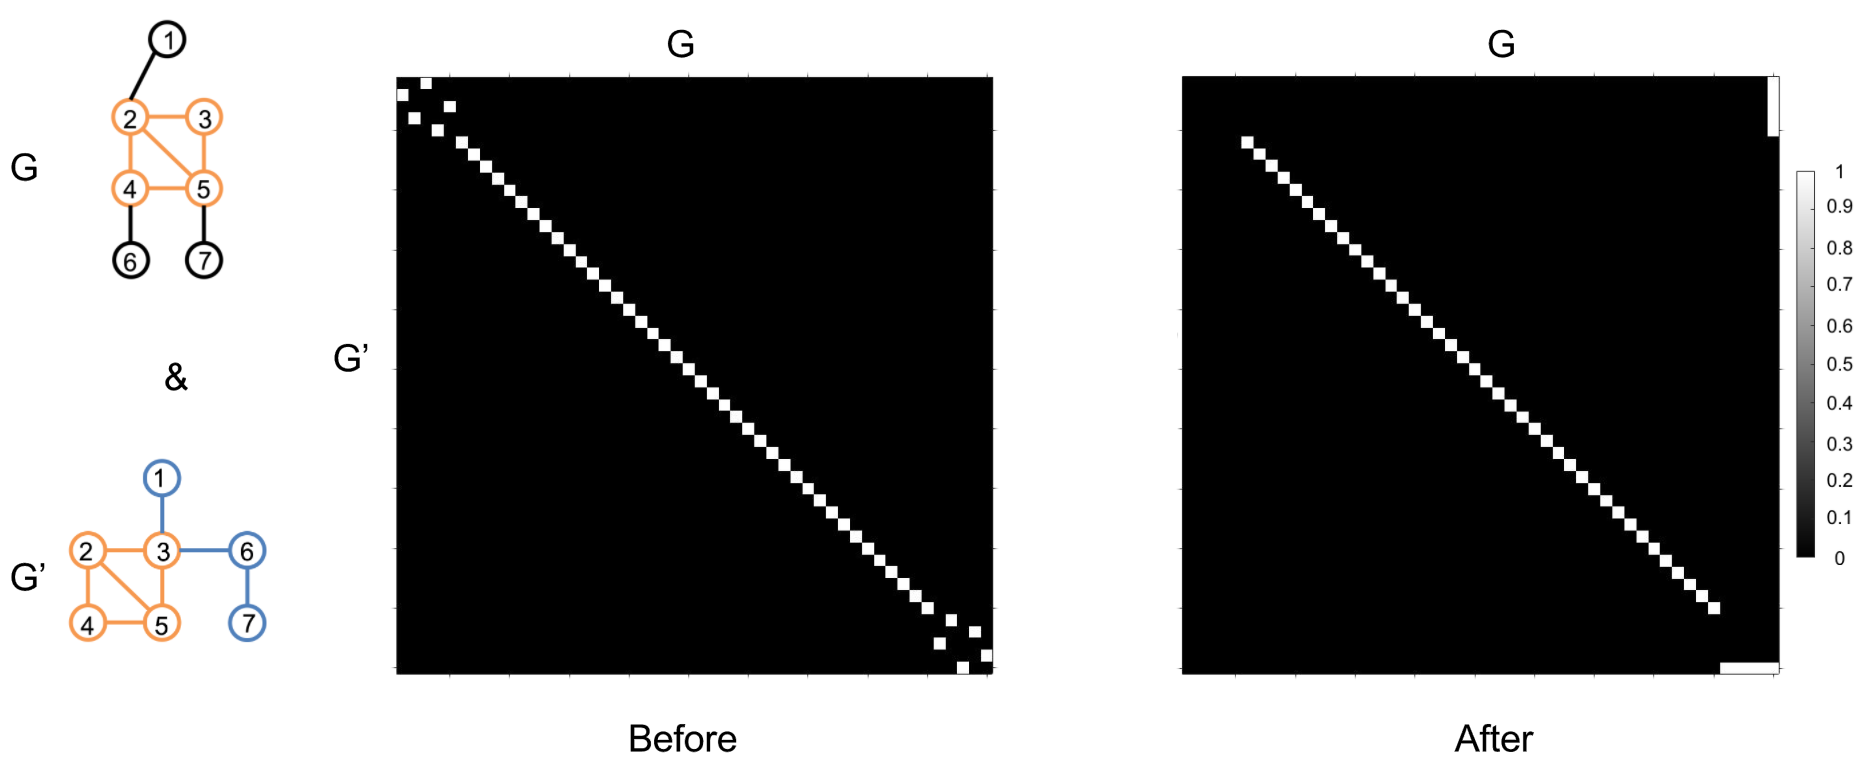
\includegraphics[width=0.8\textwidth]{figs/null_node_improve.png}
	\caption[Caption for LOF]{\emph{This is a visualization of the match matrixes produced by the original algorithm by Gold and Rangarajan (left) and the modified version (right).}}
	\label{fig:null_node_improve}
\end{figure}

\section{Conclusion}


In this chapter we introduced a graph matching algorithm that we improved and used to match the common sub-graph of two ARGs. If we do not apply the heuristic function, the match matrix $M$ shows us how likely one node in graph $G$ can be matched to another graph $G'$, which can in turn help us the summarize the common pattern among a set of graphs.

